\section{Results}




\begin{frame}{Quantitative Results 22-days ahead}
    
\begin{table}[H]
\centering
\resizebox{10cm}{!}{
\begin{tabular}{llccccccccc}
\toprule
\textbf{Dataset} & \textbf{Metric} & \textbf{n\_datasets} & \textbf{p\_value} & \textbf{Significant} & \textbf{Best Model} & \textbf{IMV-LSTM} & \textbf{XGB} & \textbf{HAR} & \textbf{GARCH} & \textbf{Stacking LSTM} \\ 
\midrule
\multirow{5}{*}{Tech} 
 & mse  & 27 & $5.80e^{-9}$ & True & stacking\_lstm & 2.81 & 2.30 & 3.56 & 5.00 & 1.33 \\ 
 & rmse & 27 & $3.21e^{-9}$ & True & stacking\_lstm & 2.74 & 2.52 & 3.52 & 5.00 & 1.22 \\ 
 & mae  & 27 & $2.04e^{-8}$ & True & stacking\_lstm & 2.70 & 2.33 & 3.56 & 5.00 & 1.41 \\ 
 & mape & 27 & $5.25e^{-8}$ & True & stacking\_lstm & 2.96 & 2.63 & 3.26 & 5.00 & 1.15 \\ 
 & smape& 27 & $8.23e^{-8}$ & True & stacking\_lstm & 2.78 & 2.63 & 3.48 & 5.00 & 1.11 \\ 
\midrule
\multirow{5}{*}{Healthcare} 
 & mse  & 23 & $4.40e^{-8}$ & True & stacking\_lstm & 2.52 & 3.43 & 2.91 & 4.87 & 1.26 \\ 
 & rmse & 23 & $1.07e^{-8}$ & True & stacking\_lstm & 2.61 & 3.35 & 2.91 & 5.00 & 1.13 \\ 
 & mae  & 23 & $5.08e^{-7}$ & True & stacking\_lstm & 2.57 & 3.48 & 2.83 & 5.00 & 1.13 \\ 
 & mape & 23 & $2.95e^{-7}$ & True & stacking\_lstm & 2.57 & 3.78 & 2.65 & 4.96 & 1.04 \\ 
 & smape& 23 & $3.74e^{-7}$ & True & stacking\_lstm & 2.57 & 3.57 & 2.87 & 5.00 & 1.00 \\ 
\midrule
\multirow{5}{*}{Industrial} 
 & mse  & 25 & $1.71e^{-8}$ & True & stacking\_lstm & 2.32 & 3.56 & 3.00 & 4.96 & 1.16 \\ 
 & rmse & 25 & $2.09e^{-8}$ & True & stacking\_lstm & 2.28 & 3.88 & 2.72 & 5.00 & 1.12 \\ 
 & mae  & 25 & $6.86e^{-7}$ & True & stacking\_lstm & 2.36 & 3.64 & 2.96 & 5.00 & 1.04 \\ 
 & mape & 25 & $5.34e^{-7}$ & True & stacking\_lstm & 2.56 & 3.88 & 2.40 & 5.00 & 1.16 \\ 
 & smape& 25 & $1.65e^{-7}$ & True & stacking\_lstm & 2.32 & 3.76 & 2.76 & 5.00 & 1.16 \\ 
\bottomrule
\end{tabular}}
\end{table}


\begin{table}[H]
\centering
\resizebox{10cm}{!}{
\begin{tabular}{c|ccccc}
\multicolumn{6}{c}{\textbf{RMSE}} \\ \hline
& imv\_lstm & xgb & har & garch & stacking\_lstm \\ \hline
imv\_lstm   & 1.000000 & 9.857569e-01 & 0.3691688 & 1.512552e-06 & 3.824534e-03 \\
xgb             & 0.985757 & 1.000000e+00 & 1.372807e-01 & 8.080748e-08 & 2.181744e-02 \\
har         & 0.369169 & 1.372807e-01 & 1.000000e+00 & 5.218468e-03 & 9.453348e-07 \\
garch       & 0.000002 & 8.080748e-08 & 5.218468e-03 & 1.000000e+00 & 1.110223e-16 \\
stacking\_lstm  & 0.003825 & 2.181744e-02 & 9.453348e-07 & 1.110223e-16 & 1.000000e+00 \\
\end{tabular}}
\end{table}


    
\end{frame}




\begin{frame}{Qualitative Results - Variable importance}
    

\begin{table}[H]
\centering
\scriptsize
\caption{Top 10 ranked features on average by sector - IMV\_LSTM variable attention}
\resizebox{9cm}{!}{
\begin{tabular}{lccc}
\toprule
\textbf{Feature Rank} & \textbf{Healthcare} & \textbf{Industrial} & \textbf{Tech} \\
\midrule
Top 1  & realized\_vol  & realized\_vol & realized\_vol \\
Top 2  & log\_return  & log\_return & log\_return \\
Top 3  & vix\_price  & eu\_term\_spread & vix\_price \\
Top 4  & volume & vix\_price & realized\_vol\_sma\_5 \\
Top 5  &  realized\_vol\_sma\_5  & volume & volume \\
Top 6  & realized\_vol\_sma\_22 & realized\_vol\_sma\_22 & rv\_vol\_5d \\
Top 7  & rv\_max\_22d & crude\_oil\_f\_price & realized\_vol\_sma\_22 \\
Top 8  & rv\_vol\_5d & realized\_vol\_sma\_5 & eu\_term\_spread \\
Top 9  & eu\_term\_spread & macd\_histogram & default\_return\_eu \\
Top 10 & macd\_histogram & ip\_eu & 1year\_expected\_inflation \\
\bottomrule
\end{tabular}}
\end{table}



\begin{table}[H]
\centering
\scriptsize
\caption{Top 10 ranked features on average by sector - HAR coefficients}
\resizebox{8cm}{!}{
\begin{tabular}{lccc}
\toprule
\textbf{Feature Rank} & \textbf{Healthcare} & \textbf{Industrial} & \textbf{Tech} \\
\midrule
Top 1  & realized\_vol  & realized\_vol & realized\_vol \\
Top 2  & realized\_vol\_sma\_5  & realized\_vol\_sma\_5 & realized\_vol\_sma\_5 \\
Top 3  & realized\_vol\_sma\_22  & realized\_vol\_sma\_22 & realized\_vol\_sma\_22 \\
Top 4  & log\_return & log\_return & log\_return \\
Top 5  & rv\_vol\_5d  & volume & rv\_vol\_5d \\
Top 6  & vix\_price & vix\_price & is\_startofweek \\
Top 7  & volume & rv\_vol\_5d & vix\_price \\
Top 8  & is\_startofweek &  rv\_vol\_22d & volume \\
Top 9  & eu\_term\_spread & is\_startofweek & rv\_vol\_22d \\
Top 10 & rv\_vol\_22d & eu\_term\_spread & default\_return \\
\bottomrule
\end{tabular}}
\end{table}


\end{frame}





\begin{frame}{Qualitative Results - Temporal importance}

\begin{figure} [H]
    \centering
    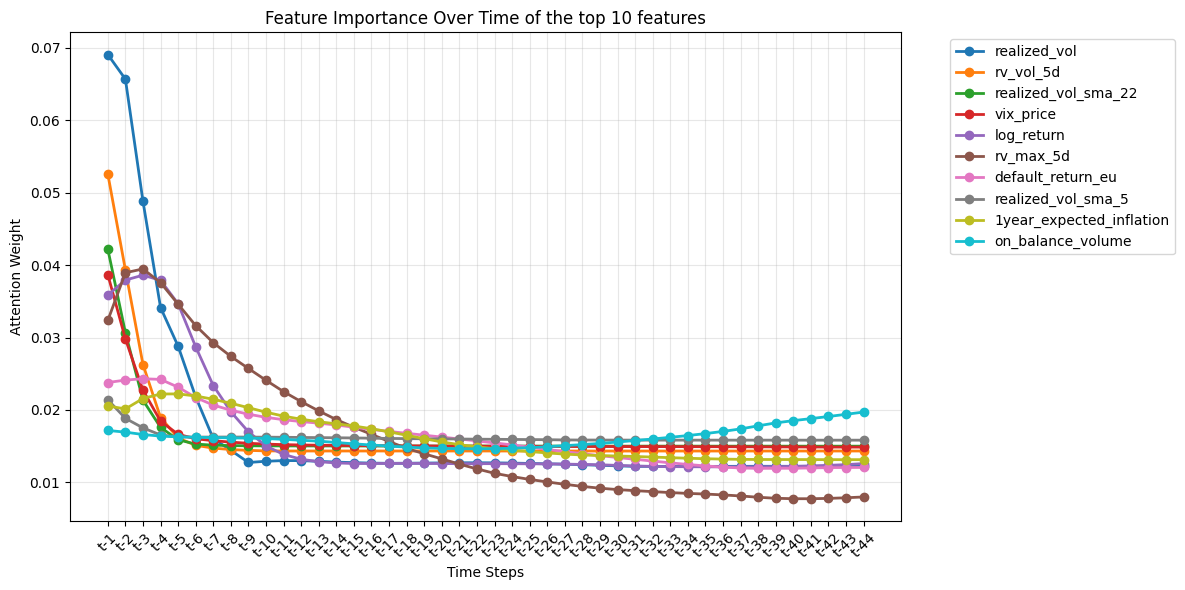
\includegraphics[scale=0.35]{images/lstm_feat_imp_over_time.png}
    \end{figure}


\end{frame}


\begin{frame}{ASML RV prediction - HAR and IMV\_LSTM}

    \begin{figure} [H]
    \centering
    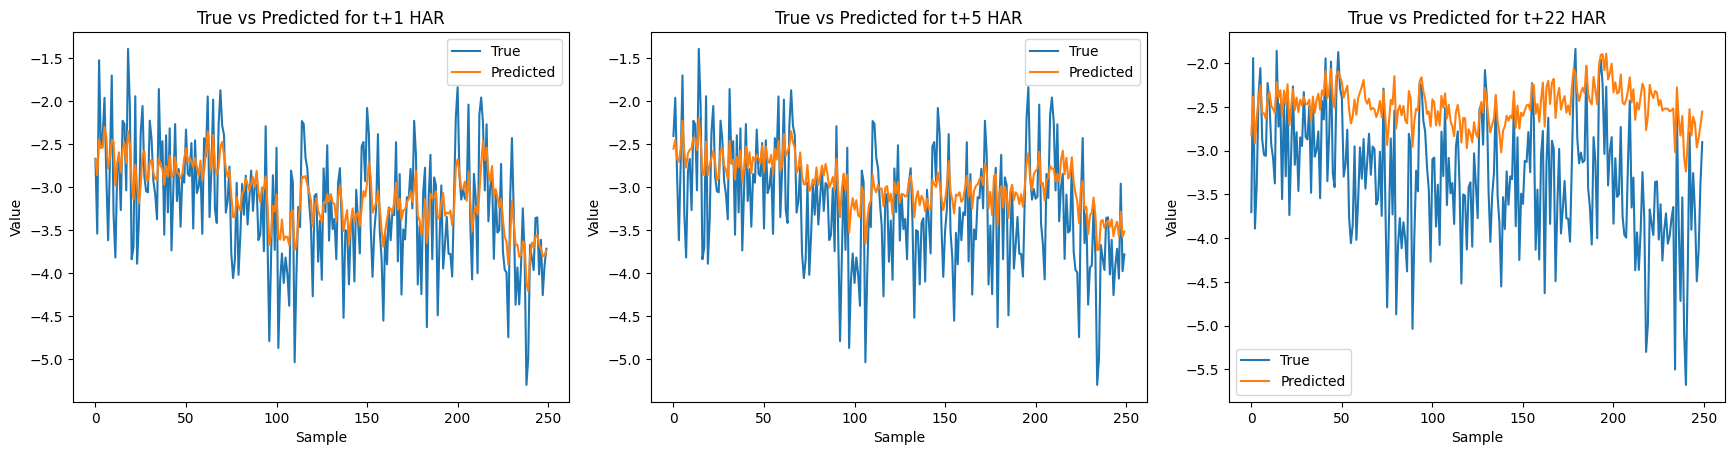
\includegraphics[scale=0.20]{images/har_pred.png}
    \end{figure}


    \begin{figure} [H]
    \centering
    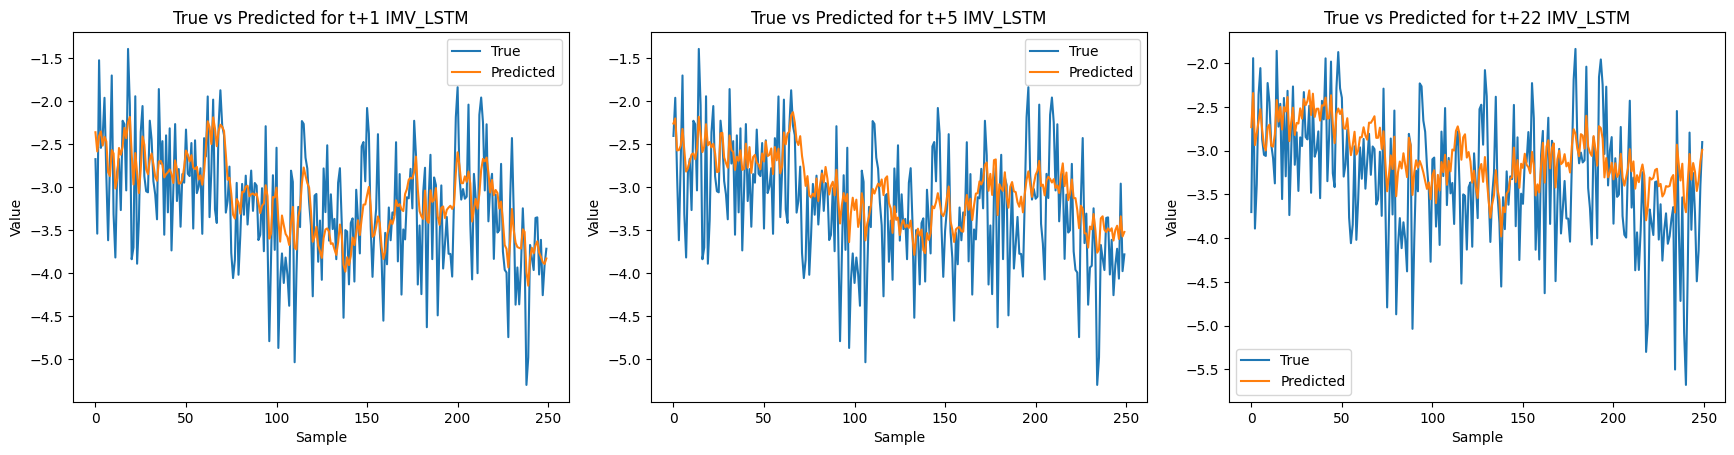
\includegraphics[scale=0.20]{images/lstm_pred.png}
    \end{figure}


    

    
\end{frame}




\begin{frame}{ASML RV prediction - Stacking Ensemble}

    

    \begin{figure} [H]
    \centering
    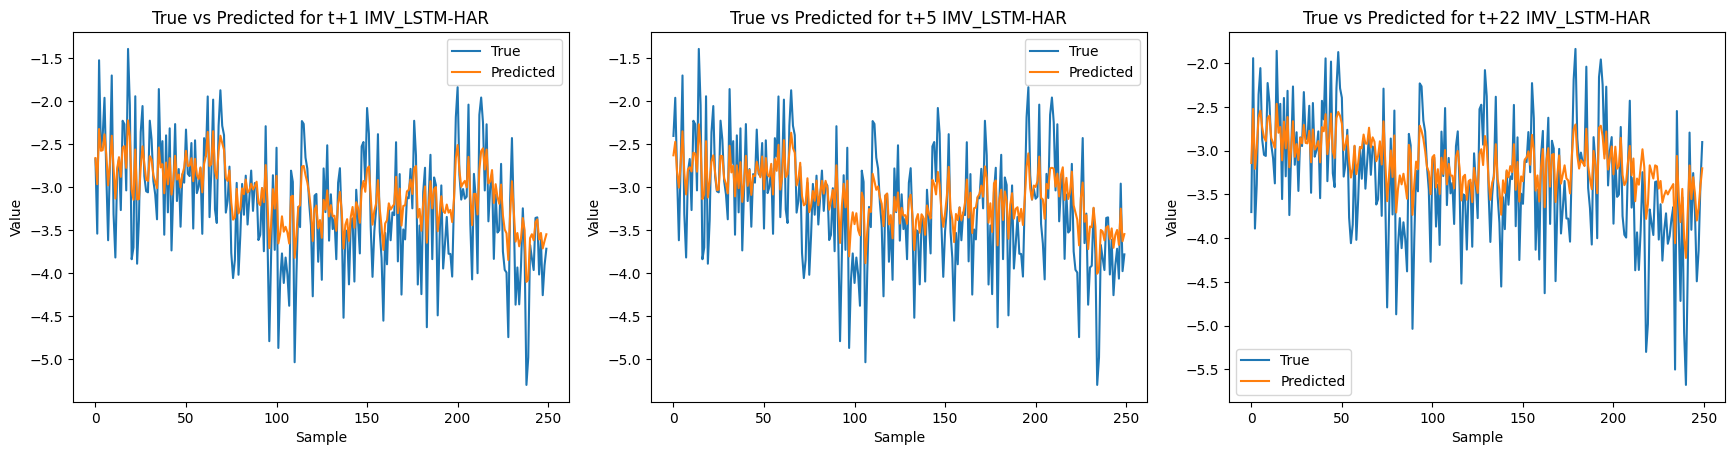
\includegraphics[scale=0.20]{images/ensemble_pred.png}
    \end{figure}


    
\end{frame}

{
\setbeamercolor{background canvas}{bg=unipi}
\begin{frame}[plain,noframenumbering]
\centering
\vfill
{\Huge\color{white}\bfseries Thank You!}
\vfill
\end{frame}
}



\begin{frame}{Sentiment Indicators}
\begin{itemize}
    \item FinSen dataset contains over than 160,000 records of Financial news from 2007 up to 2023
    \item Google news API integrates the last 2 years 
    \item FinBERT extract sentiment label $l \in [-1, 0, +1]$ and the relative probabilities $p^{(-1)}, p^{(0)}, p^{(+1)} \in P$
    \item Confidence factor is built as $c = p_1 - p_2$ where $p_1 = max P $ and $p_2 = max (P - \{p_1\})$
    \item The sentiment for a single financial headline is $s_i = l \times c$
    \item The sentiment for a single day is $S =\frac{1}{n} \sum_{i=1}^n s_i $, or 0 if no news are given for that day.
\end{itemize}

\begin{table}[h!]
\centering
\begin{tabular}{lcccc}
\hline
\textbf{Class} & \textbf{Precision} & \textbf{Recall} & \textbf{F1-Score} & \textbf{Support} \\
\hline
-1 (Negative) & 0.65 & 0.72 & 0.67 & 27 \\
0 (Neutral)   & 0.80 & 0.54 & 0.65 & 44 \\
1 (Positive)  & 0.61 & 0.76 & 0.66 &  29\\
\hline
\textbf{Accuracy}    &      &      & 0.69 & 100 \\
\textbf{Macro Avg}   & 0.69 & 0.67 & 0.66 & 100 \\
\textbf{Weighted Avg}& 0.70 & 0.65 & 0.66 & 100 \\
\hline
\end{tabular}
\end{table}

\end{frame}
